\documentclass{article}
\usepackage{tikz}
\usetikzlibrary{arrows, shapes, positioning}
\tikzstyle{nodeobserved} = [circle, minimum size = 10mm, thick, draw =black!80]
\usetikzlibrary{external}
\tikzexternalize

\begin{document}

\begin{figure}
    \begin{center}
        \tikzsetnextfilename{dag-birthweight}
        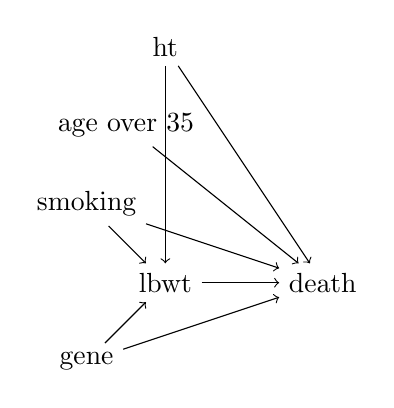
\begin{tikzpicture}
            \node (age) at (-1.5, 2) {age over 35};
            \node (smoking) at (-2, 1) {smoking};
            \node (ht) at (-1, 3) {ht};
            \node (gene) at (-2, -1) {gene};
            \node (lbwt) at (-1, 0) {lbwt};
            \node (death) at (1, 0) {death};

            \draw[->] (smoking) -- (lbwt);
            \draw[->] (ht) -- (lbwt);
            \draw[->] (gene) -- (lbwt);
            \draw[->] (gene) -- (death);
            \draw[->] (lbwt) -- (death);
            \draw[->] (smoking) -- (death);
            \draw[->] (ht) -- (death);
            \draw[->] (age) -- (death);
        \end{tikzpicture}
    \end{center}
\end{figure}

\begin{figure}
    \begin{center}
        \tikzsetnextfilename{dag-birthweight2}
        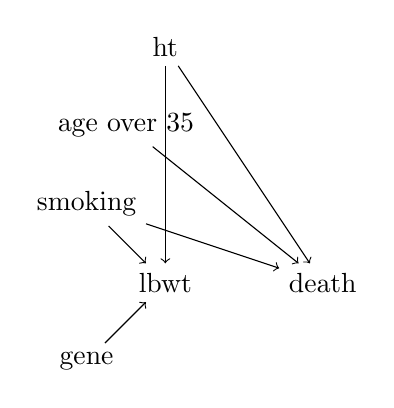
\begin{tikzpicture}
            \node (age) at (-1.5, 2) {age over 35};
            \node (smoking) at (-2, 1) {smoking};
            \node (ht) at (-1, 3) {ht};
            \node (gene) at (-2, -1) {gene};
            \node (lbwt) at (-1, 0) {lbwt};
            \node (death) at (1, 0) {death};

            \draw[->] (smoking) -- (lbwt);
            \draw[->] (ht) -- (lbwt);
            \draw[->] (gene) -- (lbwt);
            \draw[->] (smoking) -- (death);
            \draw[->] (ht) -- (death);
            \draw[->] (age) -- (death);
        \end{tikzpicture}
    \end{center}
\end{figure}

\begin{figure}
    \centering
    \tikzsetnextfilename{daga}
    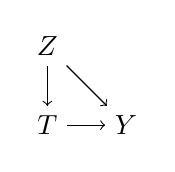
\begin{tikzpicture}
          \node (z) at (-1, 1) {$Z$};
          \node (t) at (-1, 0) {$T$};
          \node (y) at (0, 0) {$Y$};

          % Edges
          \draw[->] (z) -- (y);
          \draw[->] (z) -- (t);
          \draw[->] (t) -- (y);
    \end{tikzpicture}
\end{figure}

\begin{figure}
    \centering
    \tikzsetnextfilename{dagb}
    \begin{tikzpicture}
          \node (z) at (-1, 1) {$Z$};
          \node (t) at (-1, 0) {$T$};
          \node (y) at (0, 0) {$Y$};

          % Edges
          \draw[->] (z) -- (t);
          \draw[->] (t) -- (y);
    \end{tikzpicture}
\end{figure}

\begin{figure}
    \centering
    \tikzsetnextfilename{dagc}
    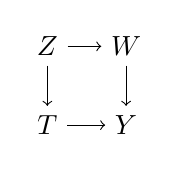
\begin{tikzpicture}
          \node (z) at (-1, 1) {$Z$};
          \node (w) at (0, 1) {$W$};
          \node (t) at (-1, 0) {$T$};
          \node (y) at (0, 0) {$Y$};

          % Edges
          \draw[->] (z) -- (w);
          \draw[->] (z) -- (t);
          \draw[->] (t) -- (y);
          \draw[->] (w) -- (y);
    \end{tikzpicture}
\end{figure}

\end{document}
